\chapter{Application to a dynamically twisted null point}
\label{chp:null_point_khi}

\graphicspath{{images/null_point_khi/}}

\section{Introduction}

This chapter presents the results of a series of numerical experiments intended to develop an understanding of the effect of anisotropic viscosity on the Kelvin-Helmholtz instability (KHI) in the fan plane of a magnetic null point, reproducing and extending the work of Wyper \& Pontin~\cite{wyperKelvinHelmholtzInstabilityCurrentvortex2013}. The numerical experiment takes the form of the dynamic twisting of an initially static magnetic null point at the footpoints of its spines, resulting in a current-vortex sheet forming in the fan plane which, given appropriate parameter choices, can be unstable to the KHI. In the course of twisting the null point, it is discovered that continued driving past the point at which the KHI occurs causes the null to spontaneously undergo spine-fan reconnection and collapse. The evolution of the KHI and the eventual collapse of the null is found to depend strongly on the form of viscosity.

The KHI has been well studied in MHD (see~\cite{faganelloMagnetizedKelvinHelmholtz2017} for a recent review and~\cite{chandrasekharHydrodynamicHydromagneticStability1981} for the classical treatment) and has been found in a number of coronal contexts, both in numerical simulations~\cite{howsonEffectsResistivityViscosity2017,wyperKelvinHelmholtzInstabilityCurrentvortex2013} and in observations~\cite{foullonMAGNETICKELVINHELMHOLTZINSTABILITY2011,yangObservationKelvinHelmholtz2018}.  In general, the effect of a magnetic field is stabilising; when the wavevector of a perturbation in a shear layer is parallel or at an oblique angle to a magnetic field, magnetic tension acts to stabilise the KHI~\cite{chandrasekharHydrodynamicHydromagneticStability1981,ryuMagnetohydrodynamicKelvinHelmholtzInstability2000}. Otherwise, the KHI acts as an interchange instability and the magnetic field does not affect its linear stability~\cite{chandrasekharHydrodynamicHydromagneticStability1981}.

In the case where a velocity shear coincides with a magnetic shear, forming a current-vortex sheet, the balance of shear layer strengths and thickness dictates if the KHI, tearing instability, or some mixture, is excited. Generally, when the magnetic shear is strong compared to the velocity shear, the KHI is suppressed and the tearing instability grows~\cite{einaudiResistiveInstabilitiesFlowing1986}. The nonlinear development of the KHI is known to enhance reconnection by local distortion of magnetic field lines and generation of current sheets~\cite{minEffectsMagneticReconnection1997} and by generating local turbulence in conjunction with the tearing instability~\cite{kowalKelvinHelmholtzTearingInstability2020}.

The effect of (anisotropic) viscosity on the stability of a current-vortex sheet is to suppress the growth of the KHI, although viscosity is found to enhance the linear growth of the tearing instability, where the KHI is stabilised by a strong magnetic field~\cite{einaudiResistiveInstabilitiesFlowing1989}. A number of studies suggest isotropic viscosity can also slow and even suppress the KHI~\cite{howsonEffectsResistivityViscosity2017,roedigerViscousKelvinHelmholtzInstabilities2013a,wyperKelvinHelmholtzInstabilityCurrentvortex2013}.

Magnetic null points, locations in a magnetic field where the field strength goes to zero, are an abundant feature in the topologically complex coronal magnetic field~\cite{edwardsNullPointDistribution2015}. Given that they are sites coinciding with changes in topology, they are strongly associated with reconnection processes~\cite{yangImagingSpectralStudy2020,sunHOTSPINELOOPS2013}. Additionally they are inferred to participate in a number of high-energy phenomena such as in the generation of flare ribbons in compact solar flares~\cite{massonNATUREFLARERIBBONS2009,pontinWhyAreFlare2016a}, production of jets~\cite{moreno-insertisPLASMAJETSERUPTIONS2013} and of coronal mass ejections (CMEs)~\cite{barnesRelationshipCoronalMagnetic2007,zouContinuousNullPointMagnetic2020}, particularly through their necessary involvement in the breakout model of eruptive solar flares~\cite{macleanTopologicalAnalysisMagnetic2005}.

A well studied form of reconnection in 3D null points is spine-fan reconnection, where a strong current sheet forms in the vicinity of the null point and enables efficient reconnection between the magnetic field making up the spine and fan plane, collapsing the field around the null in the process~\cite{thurgoodImplosiveCollapseMagnetic2018}. The collapse of a null point has the potential to develop into a form of oscillatory reconnection~\cite{thurgoodThreedimensionalOscillatoryMagnetic2017}.

The layout of this chapter is as follows. The numerical setup of the simulations is presented in Section~\ref{sec:khi_numerical_setup}, including a description of the model of linear null point and the driver used. The methods of calculating the stability measures, shear layer properties and reconnection rate are described in Section~\ref{sec:khi_analysis}. In the first part of Section~\ref{sec:khi_results} the results of a high-resolution pair of simulations are presented for a single choice of viscosity and resistivity parameters and the effect of the viscosity model compared. In the second part, the results of a parameter study are presented, generalising the high-resolution results. The chapter concludes with a discussion of findings in Section~\ref{sec:khi_discussion} and conclusions in Section~\ref{sec:khi_conclusions}.

\section{Numerical setup}

\label{sec:khi_numerical_setup}

The magnetic structure of the null point with the spine aligned along the $z$-axis is written in non-dimensional units as
\begin{equation}
  \label{eq:null_point_field}
  \vec{B} = (x, y, -2z).
\end{equation}
The non-dimensionalisation scheme is identical to that used in chapter~\ref{chp:kink_instability}. The domain is a box of dimension $[-3.5, 3.5]\times[-3.5, 3.5]\times [-0.25, 0.25] $ in the $x$, $y$ and $z$ directions, respectively. The initial velocity is uniformly zero, the initial density is uniformly $\rho = 1$ and the internal energy is uniformly $\varepsilon = 5/4$, corresponding to a temperature of $1.44 \times 10^9$K and a plasma beta of $\beta \approx 0.017$.

\begin{figure}[t]
  \centering
      \includegraphics[width=0.5\linewidth]{field_line_plots/cropped/v-4r-4-isotropic_0008_cropped.png}
  %\caption{Field lines at $t=4$ with start points anchored at a radius of $0.05$ around the spine, with the magnitude of the velocity driver shown as a slice. At this time the driver has reached its final maximum velocity of $u_0 = 0.5$. The spines of the null point already show an appreciable degree of twist.}%
  \caption{Field lines at $t=4$ showing the result of the driver, the speed of which is shown as a slice.}%
  \label{fig:field_line_plots/v-4r-4-iso-field-8}
\end{figure}

The velocity driver at the upper and lower boundaries is of an identical functional form to that used in chapter~\ref{chp:kink_instability_straight} but with modified driver parameters of $u_0 = 0.09$, $u_{r0} = 5.56$, $t_r = 0.25$ and $r_d = 36$. The peak velocity after the ramping time is $u_0$. The driver twists the footpoints of the upper and lower spines of the null point, dragging the field and introducing twist throughout the entire null point (figure~\ref{fig:field_line_plots/v-4r-4-iso-field-8}). This field and driver is similar to the setup of Wyper and Pontin~\cite{wyperKelvinHelmholtzInstabilityCurrentvortex2013}.

Unlike previous chapters, here the Braginskii-inspired parallel function~\ref{eq:alt_switching1} is used with the general switching model~\ref{eq:switching_model} to avoid the numerical cut-off associated with the spline representation of the von Mises function~\ref{eq:switching_function}. In tests it was found that the sharp transition where the von Mises function transitions to fully anisotropic (see section~\ref{sec:switching_function}) was exciting a small perturbation and disrupting the results. The parallel Braginskii switching function does not suffer from this issue.

The main parameter study required 18 simulations to be run in total; one per viscosity model for each of the 9 parameter choices. As a result a relatively low resolution of $320$ grid points in each direction is used for these runs. A higher resolution pair of simulations were run for each viscosity model at the resolution of $640$ grid points. As well as forming the basis for a detailed analysis, these higher-resolution simulations provide evidence that the lower resolution simulations have suitably converged.

\section{Tools of analysis}

\label{sec:khi_analysis}

\subsection{Shear layer properties}

To quantify the differences between the shear layers produced using different viscosity models, the peak vorticity and current density within the current-vortex sheets are measured, along with the radii at which the peaks occur. These radii are then used as the locations at which the absolute difference in azimuthal velocity $\Delta u$ and magnetic field $\Delta B$ across the shear layers are measured, calculated as the difference between the maximum and minimum values of velocity or magnetic field either side of the shear layer. The distance between the maximum and minimum points gives a measurement of the thickness of the shear layers, $L_u$ and $L_B$. These measures are all used in the calculation of the stability measures discussed in the proceeding section.

\subsection{Stability measures}

\label{sec:stability_measures}

Following Wyper and Pontin~\cite{wyperKelvinHelmholtzInstabilityCurrentvortex2013}, two quantities are used in understanding the stability of the current-vortex sheet: the fast mode Mach number $M_f$, associated with the shear in velocity, and a parameter $\Lambda$ describing the balance of stability between the tearing mode and the KHI in a current-vortex sheet. The fast mode Mach number is given by
\begin{equation}
  \label{eq:mach_numbers}
  M_f = \frac{\Delta u}{\sqrt{c_s^2 + c_A^2}}
\end{equation}
where $c_s$ and $v_A$ are the local sound and Alfv\'en speeds, respectively. The parameter $\Lambda$ measures the relative strength of the velocity shear to magnetic shear and is given by
\begin{equation}
  \label{eq:khi_stability_param}
  \Lambda = \frac{L_b}{L_u} M_A^{2/3},
\end{equation}
where $M_A$ is the projected Alfv\'en Mach number
\begin{equation}
  \label{eq:alfven_mach_number}
M_A = \frac{\Delta u \sqrt{\rho}}{\Delta B}.
\end{equation}
Since the shear layer occurs in the presence of a guide field (that of the initial magnetic null point) which is not included in the linear stability study of the KHI, the difference in magnetic field $\Delta B$ is used in the Alfv\'en Mach number as opposed to the full magnetic field strength $|\vec{B}|$. In this way the Alfv\'en Mach number can be considered projected on to the shear layer. 

Plotting the radial dependence of these quantities over the shear layers gives an idea of the linear stability based on the stability analysis performed by~\cite{einaudiResistiveInstabilitiesFlowing1986}. Such an analysis predicts that a current-vortex sheet is linearly unstable to the KHI when $M_f < 2$ and $\Lambda > 1$. When $\Lambda < 1$, the analysis predicts that the sheet is unstable to the tearing instability instead. It should be noted that the analysis of~\cite{einaudiResistiveInstabilitiesFlowing1986} is 2D. The presence of the 3D guide field in the system studied here require us to use their stability criteria only as approximations.

\subsection{Reconnection rate}

The reconnection rate is calculated using the same method employed in chapter~\ref{chp:kink_instability}. In summary, the reconnection rate local to a given magnetic field line is calculated as the local parallel electric field (that is, parallel to the magnetic field) integrated along the field line. By choosing a grid of starting points and integrating along each associated field line, an image is constructed of reconnection rates projected onto the grid of field line seed points. This is used to explore the spatial distribution of reconnection. The maximum value across all seed points gives the conventionally accepted measure of reconnection rate, the maximum integrated value~\cite{galsgaardSteadyStateReconnection2011,priestNatureThreedimensionalMagnetic2003,schindlerGeneralMagneticReconnection1988}.

\section{Results}

\label{sec:khi_results}

In the first part of the results, the evolution of the high-resolution pair of simulations is presented, both performed using a resistivity of $\eta = 10^{-4}$ and viscosity $\nu = 10^{-4}$, and the effect of the two viscosity models are compared. These simulations capture the main features of the response to the driver: the formation of a current-vortex sheet in the fan plane, the appearance of counterflows, the (potential) growth of a KHI, and an eventual null collapse. This specific choice of parameters also highlights the differences between the isotropic and the switching viscosity models, mainly the suppression of the KHI in the isotropic case, and the quicker collapse of the null in the switching case. These results are then generalised to other parameter choices in the proceeding section.

\subsection{Evolution of a typical case}
\label{sec:null_point_khi_single_case}

The evolution of the high-resolution, typical cases is detailed in stages, first exploring the formation, stability and breakup of the current-vortex sheet, before investigating the collapse of the null. Then, the evolution is summarised through an analysis of the energy budget and reconnection rate in time.

\subsubsection{Formation of the current-vortex sheet}

\begin{figure}[t]
  \centering
    %\begin{tabular}[t]{cc}
    %\hline
    \begin{subfigure}{0.49\textwidth}
      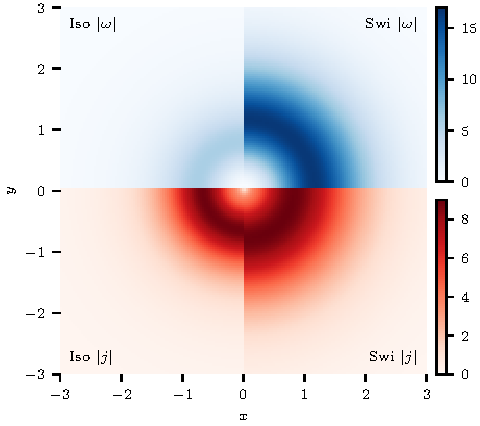
\includegraphics[width=\linewidth]{v-4r-4_vorticity_current_ring_t_3}
      \caption{Vorticity and current density rings.}
      \label{fig:v-4r-4_vorticity_current_ring_t_3}
    \end{subfigure}
    %&
    %\begin{tabular}{c}
    %\smallskip
    %\begin{subfigure}{0.49\textwidth}
      %\includegraphics[width=\linewidth]{v-4r-4_counterflows_t_3}
      %\caption{Azimuthal velocity}
      %\label{fig:v-4r-4_counterflows_t_3}
    %\end{subfigure}
    %\\
    %\begin{subfigure}{0.49\textwidth}
      %\includegraphics[width=\linewidth]{v-4r-4_lorentz_counterflows_t_3}
      %\caption{Azimuthal component of Lorentz force}
      %\label{fig:v-4r-4_lorentz_counterflows_t_3}
    %\end{subfigure}
    \hfill
    \begin{subfigure}{0.49\textwidth}
      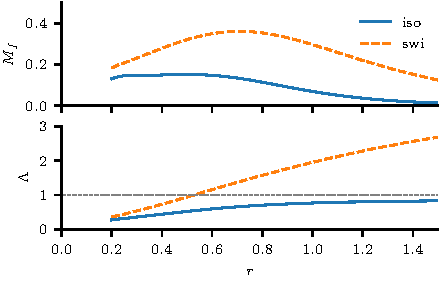
\includegraphics[width=\linewidth]{v-4r-4_mach_t_6}
      \caption{Stability measures}%
      \label{fig:v-4r-4_mach_t_6}
    \end{subfigure}
    %\end{tabular}\\
%\hline
    %\end{tabular}
\caption{Vorticity $|\omega|$ and current density $|j|$ rings and associated linear stability criteria. Subfigure (a) plots the vorticity and current density for both viscosity models at $t=3$. Subfigure (b) plots the linear stability measures as functions of radius at $t=6$. The switching model permits rings of greater radial extent and notably stronger vorticity resulting in a current-vortex sheet which is linearly unstable to the KHI.}
%\caption{Vorticity $|\omega|$ and current density $|j|$ rings and the velocity and Lorentz forces associated with the counterflows. The switching model permits rings of greater radial extent and notably stronger vorticity. Azimuthal flows counter to the relevant driver are accelerated due to the action of the magnetic tension force. All figures present data at $t=3$. Figures (b) and (c) are sliced through $x$ and show both isotropic (left of each image) and switching (right of each image) results.}
\label{fig:rings_and_stability}%
\end{figure}

Initially, the torsional Alfv\'en waves injected by the driver trace the field surrounding the null, moving first down the spines then out along the fan plane. This occurs from above and below. The upper and lower waves eventually meet and create an shear layer in the velocity and magnetic field in the form of a ring of vorticity and current density. Without any diffusion in the system the waves would travel far along the fan plane before meeting. The presence of both viscosity and resistivity diffuses the waves as they travel along the field, allowing the upper and lower waves to meet around $r=1$, creating rings of shear  (Figure~\ref{fig:v-4r-4_vorticity_current_ring_t_3}). The hole in the current-vortex sheet is due to magnetic tension forces opposing the twisting motion, as illustrated in Figure 3 of~\cite{wyperKelvinHelmholtzInstabilityCurrentvortex2013}. This also gives rise to the counterflows similar to~\cite{wyperKelvinHelmholtzInstabilityCurrentvortex2013,galsgaardNumericalExperimentsWave2003} (not shown).

In the switching case, the reduced effective viscosity produces a vortex ring which is larger in radius and stronger in magnitude. The current density ring is somewhat larger in the switching case, but of equivalent peak magnitude to that in the isotropic case. Since the viscosity diffuses velocity directly and affects the magnetic field only indirectly, the vorticity is naturally affected by the change in viscosity model more than the current density. This difference in vorticity but not current density affects the relative size of the stability measures.

Figure~\ref{fig:v-4r-4_mach_t_6} shows the relevant stability measures as functions of radius across the fan plane at $t=6$, a time when the fan plane has become unstable to the KHI in the switching case but remains stable in the isotropic case (Figure~\ref{fig:v-4r-4_uz_t_6}). The measure $\Lambda$ confirms that the current-vortex sheet is linearly stable to the KHI in the isotropic case and unstable in the switching case for $r>0.6$. This linear prediction matches where the KHI is observed to develop. In the switching case the peak of $M_f$ aligns with the observed region of initial growth of the instability.

In the switching case, $\Lambda$ and $M_f$ are significantly larger due to the enhanced velocity shear or, in other words, greater vorticity (Figure~\ref{fig:v-4r-4_vorticity_current_ring_t_3}). In the isotropic case the more efficient dissipation of velocity results in weaker vorticity and lower stability measures as a result.

%Figure~\ref{fig:v-4r-4_layers_with_time} presents the thickness and magnitudes of the velocity and magnetic shear layers as functions of time. The magnetic shear layer appears relatively unaffected by the choice of viscosity model. In contrast, the lack of viscous damping in the switching case permits a thinner velocity shear layer with a magnitude that grows faster than in the isotropic case. This combination of a thinner, stronger velocity shear layer renders the current-vortex sheet unstable to the KHI while the damping effect of isotropic viscosity reduces the shear and suppresses the instability. The larger $\Delta u$ in the switching case is reflected in the stability measure $\Lambda$ (Figure~\ref{fig:v-4r-4_mach_t_6}).

\begin{figure}[t]
  \centering
    \begin{subfigure}{0.32\textwidth}
      \includegraphics[width=\linewidth]{v-4r-4_uz_t_2}
      \caption{$t=2$}
      \label{fig:v-4r-4_uz_t_2}
    \end{subfigure}
    %\begin{subfigure}{0.32\textwidth}
      %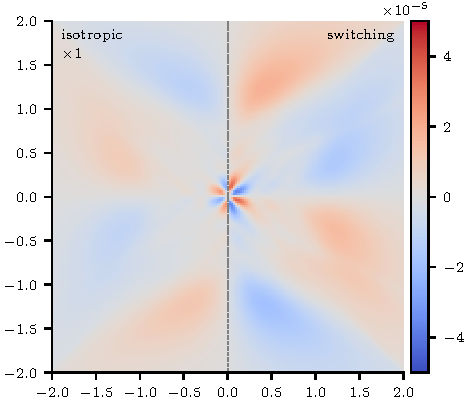
\includegraphics[width=\linewidth]{v-4r-4_uz_t_4}
      %\caption{$t=4$}
      %\label{fig:v-4r-4_uz_t_4}
    %\end{subfigure}
    \begin{subfigure}{0.32\textwidth}
      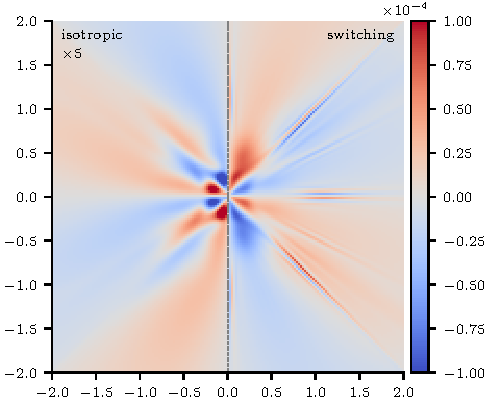
\includegraphics[width=\linewidth]{v-4r-4_uz_t_6}
      \caption{$t=6$}
      \label{fig:v-4r-4_uz_t_6}
    \end{subfigure}
    %\begin{subfigure}{0.32\textwidth}
      %\includegraphics[width=\linewidth]{v-4r-4_uz_t_8}
      %\caption{$t=8$}
      %\label{fig:v-4r-4_uz_t_8}
    %\end{subfigure}
    \begin{subfigure}{0.32\textwidth}
      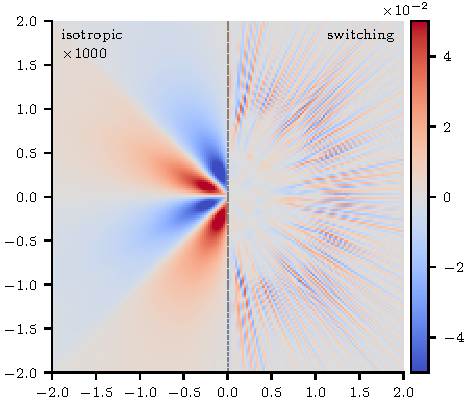
\includegraphics[width=\linewidth]{v-4r-4_uz_t_10}
      \caption{$t=10$}
      \label{fig:v-4r-4_uz_t_10}
    \end{subfigure}
    %\begin{subfigure}{0.32\textwidth}
      %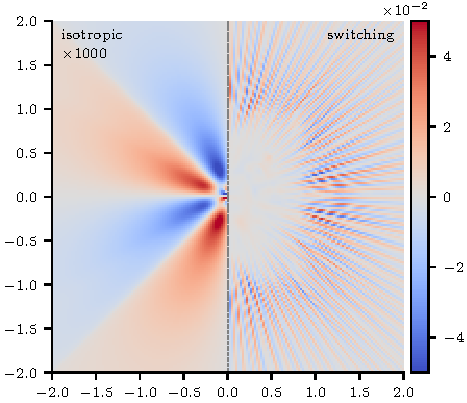
\includegraphics[width=\linewidth]{v-4r-4_uz_t_12}
      %\caption{$t=12$}
      %\label{fig:v-4r-4_uz_t_12}
    %\end{subfigure}
\caption{Out of plane velocity $u_z$ at $t=2, 6$ and $10$ for both viscosity models. Note the isotropic results have been multiplied by as much as $1000$ in order to compare to the switching results. In the switching case the KHI appears initially along the diagonals before extending azimuthally. In the isotropic case there is no evidence of the instability.}
\label{fig:out_of_plane_velocity}%
\end{figure}

As expected from the linear stability presented in Figure~\ref{fig:v-4r-4_mach_t_6}, Figure~\ref{fig:out_of_plane_velocity} shows the development of the out of plane velocity from $t=2$ to $10$ and reveals that only the current-vortex sheet in the switching case is unstable to the KHI. Both cases appear similar until $t=6$ when the KHI appears only in the switching case, initially along the diagonals (Figure~\ref{fig:v-4r-4_uz_t_6}) before spreading azimuthally (Figure~\ref{fig:v-4r-4_uz_t_10}). There is no evidence of the KHI in the isotropic case.

%\begin{figure}[t]
  %\centering
    %\begin{subfigure}{0.49\textwidth}
      %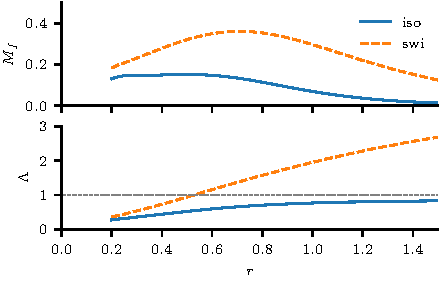
\includegraphics[width=\linewidth]{v-4r-4_mach_t_6}
      %\caption{Stability parameters}%
      %\label{fig:v-4r-4_mach_t_6}
    %\end{subfigure}
    %\hfill
    %\begin{subfigure}{0.49\textwidth}
      %\includegraphics[width=\linewidth]{v-4r-4_layers_with_time}
      %\caption{Shear layer properties}
      %\label{fig:v-4r-4_layers_with_time}
    %\end{subfigure}
%\caption{Properties of the shear layers for the isotropic case (blue, solid line) and switching case (orange, dashed line). Subfigure (a) plots the fast Mach number $M_f$ and stability measure $\Lambda$ as functions of radius $r$ at $t=6$. Subfigure (b) plots the dependence of the shear widths $L_u$ and $L_B$ and the shear magnitudes $\Delta u$ and $\Delta B$ as functions of time and at a radius of $r=0.7$. The major contributing factor to the instability of the shear layer in the switching case is the velocity shear.}
%\label{fig:v-4r-4_layers}%
%\end{figure}

\begin{figure}[t]
  \centering
    \begin{subfigure}{0.48\textwidth}
      \includegraphics[width=\linewidth]{v-4r-4_vorticity_current_ring_t_10}
      \caption{Current-vortex sheet}
      \label{fig:v-4r-4_vorticity_current_ring_t_10}
    \end{subfigure}
    \hfill
    \begin{subfigure}{0.48\textwidth}
      \includegraphics[width=\linewidth]{v-4r-4_reconn_rate_t_10}
      \caption{Reconnection rate}
      \label{fig:v-4r-4_reconn_rate_t_10}
    \end{subfigure}
\caption{The breakup of the current-vortex sheet and associated reconnection at $t=10$. Subfigure (a) presents the current and vorticity density and subfigure (b) presents the spatial distribution of reconnection rate. Both subfigures show both viscosity models. The current-vortex sheet remains stable in the isotropic case while that in the switching case has been fragmented by the KHI. The resultant small-scale reconnection in the rolls produce localised pockets of strong vorticity and current density.}
\end{figure}

In both cases the current-vortex sheet grows in radius and magnitude with time, more in the switching case than in the isotropic. The shearing action of the counterflows produces a secondary ring of strong current density closer to the spine which is greater in magnitude in the isotropic case. By $t=10$ the KHI has disrupted the current-vortex sheet (Figure~\ref{fig:v-4r-4_vorticity_current_ring_t_10}) and the resultant rolls of the KHI create strong, small-scale current sheets, enhancing the local reconnection rate. 

Figure~\ref{fig:v-4r-4_reconn_rate_t_10} shows the spatial distribution of the reconnection rate for both viscosity models. Each pixel in the image represents one field line passing through that pixel along which the parallel electric field has been integrated. The colour of the pixel is given by the value of the integration. The reconnection rate is greatest close to the origin, corresponding to regions of slippage reconnection due to the strong currents in the spine and current-vortex sheet. The effects of the boundary can be seen as long dark lines which spiral outwards from the origin. The switching case shows greater peak reconnection rate due to the small scale current sheets created by the KHI, and the enhanced reconnection far from the null can be seen as ripple-like structures in the fringes of the plot.

\subsubsection{Spine-fan reconnection}

This section presents the results of driving a magnetic null to the point at which it undergoes spontaneous collapse. The collapse is instigated by a velocity shear across the null creating a magnetic shear which allows spine-fan reconnection. The results of the isotropic case are first presented in detail, then the effect of the KHI is explored in the switching case.

\begin{figure}[t]
  \centering
    \begin{subfigure}{0.49\textwidth}
      \includegraphics[width=\linewidth]{field_line_plots/cropped/v-4r-4-isotropic_0030_cropped.png}
      \caption{$t=15$}
      \label{fig:v-4r-4-iso-field-30}
    \end{subfigure}
    \hfill
    \begin{subfigure}{0.49\textwidth}
      \includegraphics[width=\linewidth]{field_line_plots/cropped/v-4r-4-isotropic_0037_cropped.png}
      \caption{$t=18.5$}
      \label{fig:v-4r-4-iso-field-37}
    \end{subfigure}
\caption{Collapse of the null point visualised with field lines in the isotropic case. Field lines are plotted from a circle of radius $0.05$ around the upper and lower spine footpoints. Contours of $|\vec{j}| = 60$ are also plotted and reveal the strong current within the spine as well as the formation of the central sheet associated with the spine-fan reconnection. At $t=18.5$ the bulk of the field lines making up the core of the spines have reconnected.}
\label{fig:khi_field_lines_collapse}
\end{figure}

In typical studies of spine-fan reconnection (such as~\cite{pontinCurrentSheetFormation2007}) the spines of a null point are dragged in opposite directions at the boundaries. This motion pulls the field above and below the null point in opposite directions and creates a current sheet which acts to reconnect field lines between the spine and fan field lines. Here, the field near the null is shifted not because of motions at the footpoints of the spines, but due to imbalances in the velocity which arise naturally during the course of the initial driving. Figure~\ref{fig:khi_field_lines_collapse} presents the magnetic field lines before and during the reconnection.

\begin{figure}[t]
  \centering
    \begin{subfigure}{0.49\textwidth}
      \includegraphics[width=\linewidth]{v-4r-4-pressure-flow-30.pdf}
      \caption{Pressure and flow}
      \label{fig:v-4r-4-pressure-flow-30}
    \end{subfigure}
    \hfill
    \begin{subfigure}{0.32\textwidth}
      \includegraphics[width=\linewidth]{v-4r-4-vx-imbalance-30.pdf}
      \caption{Imbalance in $u_x$}
      \label{fig:v-4r-4-vx-imbalance-30}
    \end{subfigure}
    %\hfill
    %\begin{subfigure}{0.32\textwidth}
      %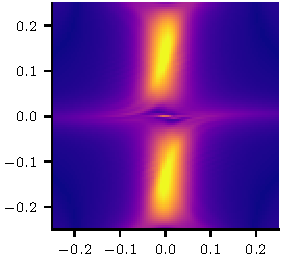
\includegraphics[width=\linewidth]{v-4r-4-spine-fan-reconn-35.pdf}
      %\caption{$t=17.5$}
      %\label{fig:v-4r-4-spine-fan-reconn-35}
    %\end{subfigure}
\caption{Velocity imbalance above and below the null. Figure (a) plots a slice of the pressure through $y=0$ overlaid with fluid velocity, where the longest arrows correspond to a fluid velocity of approximately $0.1$. Figure (b) depicts $|u_x(x)| - |u_x(-x)|$, the difference in $u_x$ between the left and right sides of the plane $x=0$. This gives a measure of the asymmetry in the velocity around the null point.}
\label{fig:imbalance_in_velocity}
\end{figure}

The twist in the spines creates a current which heats the contained plasma via Ohmic heating and generates a small pressure force directed towards the null point. This drives two oppositely directed streams of plasma down the spines towards the null point (Figure~\ref{fig:v-4r-4-pressure-flow-30}). Where these streams meet at the null point, they form a stagnation point flow, compressing the plasma in the vicinity of the null and flowing out along the fan plane. Due to small asymmetries in the solution that accrue during the course of the simulation, an imbalance in the velocity appears above and below the null point (Figure~\ref{fig:v-4r-4-vx-imbalance-30}). 

\begin{figure}[t]
  \centering
    \begin{subfigure}{0.32\textwidth}
      \includegraphics[width=\linewidth]{v-4r-4-spine-fan-reconn-34.pdf}
      \caption{$t=17$}
      \label{fig:v-4r-4-spine-fan-reconn-34}
    \end{subfigure}
    \hfill
    \begin{subfigure}{0.32\textwidth}
      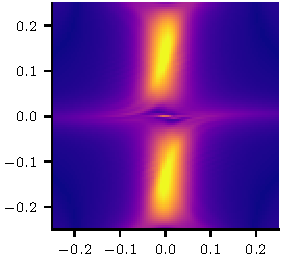
\includegraphics[width=\linewidth]{v-4r-4-spine-fan-reconn-35.pdf}
      \caption{$t=17.5$}
      \label{fig:v-4r-4-spine-fan-reconn-35}
    \end{subfigure}
    \hfill
    \begin{subfigure}{0.32\textwidth}
      \includegraphics[width=\linewidth]{v-4r-4-spine-fan-reconn-36.pdf}
      \caption{$t=18$}
      \label{fig:v-4r-4-spine-fan-reconn-36}
    \end{subfigure}
\caption{Development of the spine-fan reconnection current sheet shown as plots of $|\vec{j}|$ sliced through $y=0$ between $t=17$ and $18$. Maximum current density in all plots is $|\vec{j}| = 120$.}
\label{fig:spine_fan_reconnection_current_sheet}
\end{figure}

The velocity shear around the null shears the magnetic field accordingly, creating a current sheet through the null point in the process (Figures~\ref{fig:spine_fan_reconnection_current_sheet}). The current sheet enables reconnection between the spine and fan which further extends, thins and strengthens the sheet, continuing the reconnection process (Figure~\ref{fig:v-4r-4-iso-field-37}) until the field around the null collapses. The collapse itself can be seen in the kinetic energy as a dramatic increase starting at $t\approx18$ (Figure~\ref{fig:v-4r-4_kinetic_energy}). The development of the current sheet and the resultant spine-fan reconnection is similar to that of~\cite{pontinCurrentSheetFormation2007} with the exception that the twist in the field unravels as the reconnection proceeds. 

In the switching case, the development of the spine-fan reconnection and associated collapse is qualitatively similar to that in the isotropic case with the exception that the reconnection occurs notably earlier. Where the current sheet development shown in Figures~\ref{fig:spine_fan_reconnection_current_sheet} occurs between $t=17$ and $18$ in the isotropic case, a similar evolution occurs between $t=14$ and $15$ in the switching.

\subsubsection{Overview of current-vortex sheet development and null collapse}

\begin{figure}[t]
  \centering
  \begin{subfigure}{0.32\textwidth}
    \includegraphics[width=\linewidth]{v-4r-4_kinetic_energy}
    \caption{Kinetic energy}
    \label{fig:v-4r-4_kinetic_energy}
  \end{subfigure}
  \hfill
  \begin{subfigure}{0.32\textwidth}
    \includegraphics[width=\linewidth]{v-4r-4_viscous_heating}
    \caption{Viscous heating}%
    \label{fig:v-4r-4_viscous_heating}
  \end{subfigure}
  \hfill
  \begin{subfigure}{0.32\textwidth}
    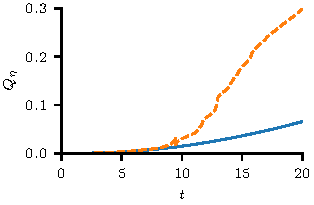
\includegraphics[width=\linewidth]{v-4r-4_ohmic_heating}
    \caption{Ohmic heating}%
    \label{fig:v-4r-4_ohmic_heating}
  \end{subfigure}
  \hfill
  \begin{subfigure}{0.32\textwidth}
    \includegraphics[width=\linewidth]{v-4r-4_magnetic_energy}
    \caption{Magnetic energy}%
    \label{fig:v-4r-4_magnetic_energy}
  \end{subfigure}
  \hfill
  \begin{subfigure}{0.32\textwidth}
    \includegraphics[width=\linewidth]{v-4r-4_internal_energy}
    \caption{Internal energy}%
    \label{fig:v-4r-4_internal_energy}
  \end{subfigure}
  \hfill
  \begin{subfigure}{0.32\textwidth}
    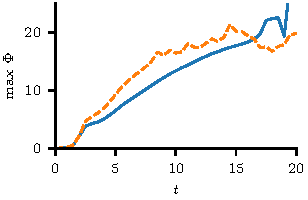
\includegraphics[width=\linewidth]{v-4r-4_reconn_rate_over_time}
    \caption{Reconnection rate}%
    \label{fig:v-4r-4_reconn_rate_over_time}
  \end{subfigure}
  \caption{Energy measures and reconnection rate as functions of time.}
  %\caption{Kinetic energy (a) and reconnection rate (b) as functions of time for the isotropic (blue, solid line) and switching (orange, dashed line) cases using diffusion parameters $\nu=10^{-4}$ and $\eta=10^{-4}$. The switching case shows clear growth of the KHI starting from $t=2$. While the isotropic case shows no evidence of the KHI, there is evidence of the null collapse at $t\approx18$. The reconnection rate reveals the nonlinear phase of the KHI as a period of bursty reconnection in the switching case and the eventual collapse in both cases.}
\end{figure}

The kinetic energy in the switching case mirrors the main evolution of a KHI-unstable current-vortex sheet as presented previously (Figure~\ref{fig:v-4r-4_kinetic_energy}). The initial injection of the Alfv\'en waves and formation of the current-vortex sheet can be seen at at $t\approx3$. As the null continues to be driven, the sheet becomes unstable to the KHI and the kinetic energy grows accordingly from $t\approx3$ to $8$. At $t\approx 8$ the KHI saturates as small-scale current sheets are formed and Ohmic heating begins to drain the energy from the instability (Figure~\ref{fig:v-4r-4_ohmic_heating}). This is also reflected in the reconnection rate, Figure~\ref{fig:v-4r-4_reconn_rate_over_time}, where the small current sheets in the fan plane promote local reconnection in the rolls of the KHI. Around $t=14$, a transient increase in the kinetic energy reveals the start of the null collapse. 

In the isotropic case, the kinetic energy increase and enhanced reconnection rate associated with the KHI is absent, however the collapse of the null produces significantly more kinetic energy at $t\approx 17$ than in the switching case (Figure~\ref{fig:v-4r-4_kinetic_energy}). The Ohmic heating is similarly damped without the influence of the KHI (Figure~\ref{fig:v-4r-4_ohmic_heating}). This results in the switching model extracting more energy from the field (Figure~\ref{fig:v-4r-4_magnetic_energy}) and heating the plasma much more efficiently (Figure~\ref{fig:v-4r-4_internal_energy}). One significant finding is that the velocity shears created by the KHI allow anisotropic viscous heating of comparable levels to that of isotropic viscosity (in contrast to the orders of magnitude difference observed in other chapters). 

The reconnection rate reveals some interesting features about the nature of reconnection within the system and how the presence of the KHI affects the null collapse (Figure~\ref{fig:v-4r-4_reconn_rate_over_time}). One interesting observation is that the switching case shows a greater reconnection rate than that of the isotropic case even before the onset of the KHI (i.e. for $t < 6$), suggesting the switching model itself is enhancing reconnection. As in other chapters, this is due to the switching model permitting greater velocities, greater compression and thinner, stronger current sheets. It is then unclear whether the generally enhanced reconnection rate in the switching case for times $t=5$--$10$ can be attributed to the current-enhancing effect of the switching model or an effect of the KHI. Certainly, the spiky nature of the reconnection rate from $t=8$--$15$ can be attributed to the small, strong current sheets produced in the rolls of the KHI, which do not appear in the stable isotropic case. The collapse of the null is observed in the reconnection rate in the switching case around $t=15$ and in the isotropic case around $t= 17$, however it differs significantly between the two cases. In the isotropic case, the reconnection rate increases during the collapse, while in the switching case, it decreases. 

\todo{replace these figs with t=20 ones}

\begin{figure}[t]
  \centering
    \begin{subfigure}{0.49\textwidth}
      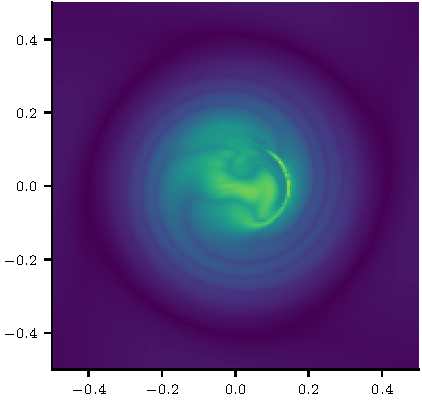
\includegraphics[width=\linewidth]{v-4r-4_reconn_rate_t_+18.5iso.pdf}
      \caption{isotropic}
      \label{fig:v-4r-4_reconn_rate_t_+18.5iso}
    \end{subfigure}
    \hfill
    \begin{subfigure}{0.49\textwidth}
      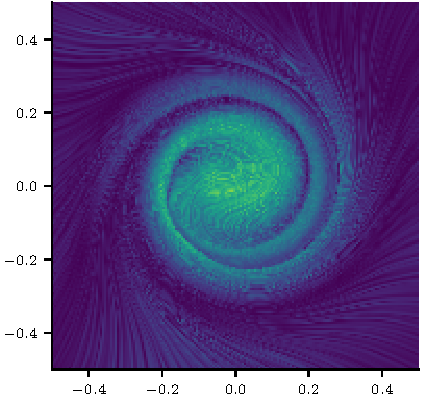
\includegraphics[width=\linewidth]{v-4r-4_reconn_rate_t_+18.5swi.pdf}
      \caption{switching}
      \label{fig:v-4r-4_reconn_rate_t_+18.5swi}
    \end{subfigure}
\caption{Difference in the spatial distribution of the reconnection rate at $t=18.5$.}
\label{fig:reconnection_rate_null_collapse}
\end{figure}

Figure~\ref{fig:reconnection_rate_null_collapse} shows the differences in spatial distribution of the reconnection rate between the two cases at $t=20$, a time when the maximum reconnection rate has increased as a result of the null collapse in the isotropic case and dropped in the switching case (Figure~\ref{fig:v-4r-4_reconn_rate_over_time}). In the isotropic case (Figure~\ref{fig:v-4r-4_reconn_rate_t_+18.5iso}) the reconnection is greatest along a thin structure indicative of the reconnection occurring in the strong current sheet at the null point (seen in Figure~\ref{fig:v-4r-4-spine-fan-reconn-36}).

Firstly, the null disrupts the reconnection-enhancing KHI which then lowers the overall reconnection rate. Secondly, the KHI generates a turbulent-like state in the fan plane which offers resistance to the collapse in a way  (which itself enhances reconnection) being disrupted by the collapse of the null in the switching case. In the isotropic case where the KHI is not present, the null collapses 

\subsection{Analysis of parameter study}

The results shown in section~\ref{sec:null_point_khi_single_case} can change dramatically when $\nu$ and $\eta$ are varied. This section presents results of simulations where $\nu$ is varied as $10^{-5}$, $10^{-4}$ or $10^{-3}$ and $\eta$ taking the values $10^{-4}$ or $10^{-3}$. This results in six pairs of simulations, each choice being run with switching viscosity or isotropic viscosity. The simulations were performed at a resolution of $320$ grid points per dimension, half that of the typical cases, and run to $t=15$ instead of $t=20$ as in the typical cases. As a result, the null collapse occurs sooner than at higher resolutions and shows behaviour more typical of fast reconnection indicative of inadequate resolution~\cite{miyamaNumericalAstrophysicsProceedings2012}. For this reason, focus remains on the development of the KHI rather than the null collapse.

Generally, increasing $\eta$ to $10^{-3}$ produces a null that is more unstable to the KHI (even in isotropic cases). Increasing $\nu$ damps the KHI but does not totally suppress it, while decreasing $\nu$ leads to a more unstable KHI. We present first the quantitative effect of varying $\nu$, $\eta$ and the viscosity models on the properties of the shear layers and the resulting stability and development of the KHI.

%As an aside, in all $\nu = 10^{-3}$ isotropic simulations there's an unexpected, transient artifact in every examined variable. This was also seen in the kink instability simulations in chapter TODO. This is assumed to be due to small-amplitude fast waves created during the initial ramp up, the interaction of which causes the isotropic viscous stress tensor to produce odd effects. It appears to only affect the first time step and the effect is only to slightly increase the viscous heating. Since the affected results don't differ wildly from those of the unaffected $\nu=10^{-4}$ simulations we cautiously trust these results.

\subsubsection{Shear layer properties and instability}

\begin{figure}[t]
    \begin{subfigure}{0.49\textwidth}
      \centering
  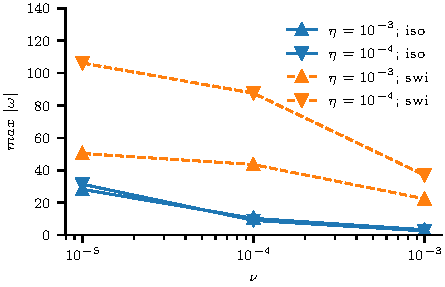
\includegraphics[width=1.0\linewidth]{param_study/peak_vort.pdf}
      \caption{Peak vorticity}%
      \label{fig:peak_vort}
    \end{subfigure}
    \hfill
    \begin{subfigure}{0.49\textwidth}
      \centering
  \includegraphics[width=1.0\linewidth]{param_study/peak_current.pdf}
      \caption{Peak current}%
      \label{fig:peak_current}
    \end{subfigure}
  \caption{Peak vorticity and current as functions of $\nu$ for each value of $\eta$ at $t=8$. In the isotropic case, both rings decrease in radial extent as either diffusion parameter is increased. In the switching case, both rings also decrease with $\eta$, however there is a notable increase in the radial extent with $\nu$, particularly for high values of $\eta$.}%
  \label{fig:param_study_peak_mag_and_loc}
\end{figure}

To understand the effect that viscosity and resistivity have on the stability of the current-vortex sheet, it is useful to understand how changing their strength affects the magnitude of the vorticity and current density rings. Figure~\ref{fig:param_study_peak_mag_and_loc} presents the peak vorticity and current density as functions of $\nu$ for both values of $\eta$. In general, increased diffusion leads to a thicker, weaker ring, due to the Alfv\'en waves diffusing more before meeting in the fan plane. This is reflected in the general trends found in figure~\ref{fig:param_study_peak_mag_and_loc}, where peak current, peak vorticity. The switching model, being generally less diffusive than the isotropic model, permits velocity shear layers with much greater peak vorticity. Due to the coupling between the magnetic field and the velocity in an Alfv\'en wave, the isotropic model appears to provide some diffusion to the magnetic field during the formation of the magnetic shear layer, resulting in a layer with weaker peak current, however the switching model affects the magnetic layer very little.

Since the stability of the current-vortex sheet depends on the balance of velocity and magnetic shear, it is not exactly clear from Figure~\ref{fig:param_study_peak_mag_and_loc} what the effect of changing resistivity is on the ultimate stability of the sheet. Lower resistivity results in a stronger vorticity layer (in the switching case) but also a stronger current layer, and vice versa for larger resistivity. To fully understand the effect of the diffusion parameters on the stability of the sheet, analysis of the sheets using the stability parameters $\Lambda$ and $M_f$ is required.

\begin{figure}[t]
    \hfill
    \begin{subfigure}{0.49\textwidth}
      \centering
  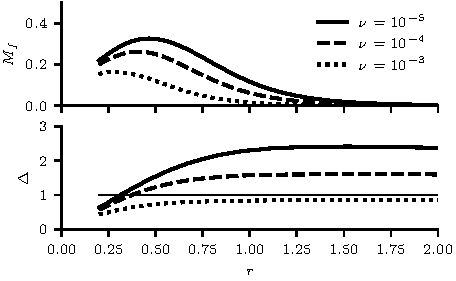
\includegraphics[width=1.0\linewidth]{param_study/mach_numbers_eta_3_iso.pdf}
      \caption{Isotropic; $\eta = 10^{-3}$}%
      \label{fig:mach_numbers_eta_3_iso}
    \end{subfigure}
    \hfill
    \begin{subfigure}{0.49\textwidth}
      \centering
  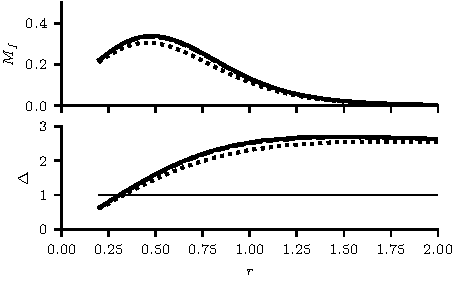
\includegraphics[width=1.0\linewidth]{param_study/mach_numbers_eta_3_swi.pdf}
      \caption{Switching; $\eta = 10^{-3}$}%
      \label{fig:mach_numbers_eta_3_swi}
    \end{subfigure}
    \hfill
    \begin{subfigure}{0.49\textwidth}
      \centering
  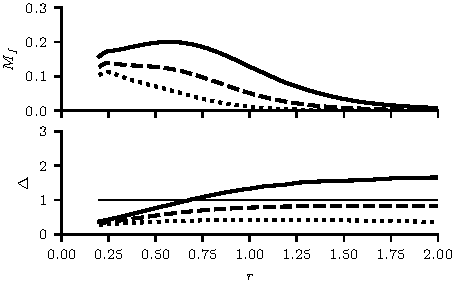
\includegraphics[width=1.0\linewidth]{param_study/mach_numbers_eta_4_iso.pdf}
      \caption{Isotropic; $\eta = 10^{-4}$}%
      \label{fig:mach_numbers_eta_4_iso}
    \end{subfigure}
    \hfill
    \begin{subfigure}{0.49\textwidth}
      \centering
  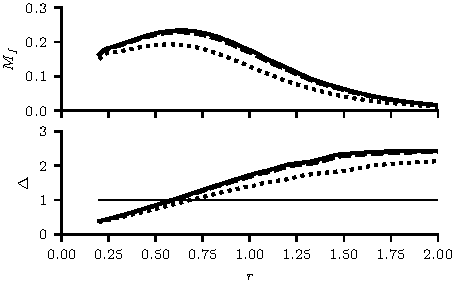
\includegraphics[width=1.0\linewidth]{param_study/mach_numbers_eta_4_swi.pdf}
      \caption{Switching; $\eta = 10^{-4}$}%
      \label{fig:mach_numbers_eta_4_swi}
    \end{subfigure}

  \caption{Plots of $M_f$ and $\Lambda$ as functions of $r$ for all parameter choices at $t=8$. Note the difference in the scale of $M_f$ for difference values of $\eta$. The cases where $\Lambda > 1$ are unstable with the exception of the isotropic cases where $\nu=10^{-4},\eta=10^{-3}$ (dashed line in figure~\ref{fig:mach_numbers_eta_3_iso}).}%
  \label{fig:mach_numbers}
\end{figure}

Figure~\ref{fig:mach_numbers} plots the stability measures as functions of radius for every studied parameter choice and both viscosity models at $t=8$. In every case $M_f < 2$, a necessary condition for an unstable current-vortex sheet. The condition on $\Lambda$ for instability is $\Lambda > 1$. All switching layers are linearly unstable to the KHI (Figures~\ref{fig:mach_numbers_eta_3_swi} and~\ref{fig:mach_numbers_eta_4_swi}) while the isotropic cases show a mix of linear stability. When $\nu = 10^{-5}$, the viscosity is weaker and the linear stability analysis predicts that the layers should be unstable for either value of $\eta$. The opposite is true for $\eta=10^{-3}$, when the isotropic viscosity is at its most dissipative. The two middle cases, when $\nu=10^{-4}$ show linear stability when $\eta=10^{-4}$ and instability when $\eta=10^{-3}$.

\begin{table}[t]
\centering
\begin{tabular}{llllllll}
$\eta$    & $\nu$     & Iso linear & Iso observed & Swi linear & Swi observed  \\
\midrule
$10^{-3}$ & $10^{-3}$ & Stable     & Stable       & Unstable   & Unstable         & \\
$10^{-3}$ & $10^{-4}$ & Unstable   & Stable       & Unstable   & Unstable         & \\
$10^{-3}$ & $10^{-5}$ & Unstable   & Unstable     & Unstable   & Unstable         & \\
$10^{-4}$ & $10^{-3}$ & Stable     & Stable       & Unstable   & Unstable*         & \\
$10^{-4}$ & $10^{-4}$ & Stable     & Stable       & Unstable   & Unstable         & \\
$10^{-4}$ & $10^{-5}$ & Unstable   & Unstable*     & Unstable   & Unstable         &
\end{tabular}
\caption{Stability in the isotopic and switching cases for different choices of $\nu$ and $\eta$. Both linear stability (as predicted by $\Lambda > 1$ in Figure~\ref{fig:mach_numbers}) and observed stability are shown. Entries marked as unstable* show growth of the KHI but the growth rate of the perturbation is close to zero. The isotropic model mostly results in stability while the switching model mostly results in instability.}
\label{tab:stability}
\end{table}

The observed stability of the current-vortex sheet to the KHI in each case is determined via inspection of the out of plane velocity for each parameter choice and is summarised for each parameter choice in table~\ref{tab:stability}. Some entries are marked as unstable*, referring to their being technically unstable (that is the KHI is directly observed in the out of plane velocity) but the growth rate is close to zero and the perturbation remains negligibly small even at the final time of $t=15$. This is well matched by the theoretical conditions of instability $\Lambda > 1$ and $M_f < 2$ in all but one case. This indicates  that despite the difference in geometry, the stability analysis of~\cite{einaudiResistiveInstabilitiesFlowing1986} is of practical use in predicting the stability of the KHI in magnetic null points. This condition even accurately predicts the stability of the marginal cases discussed previously. 

\begin{figure}[t]
  \centering
    \begin{subfigure}{0.32\textwidth}
      \centering
      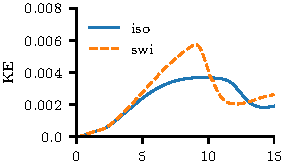
\includegraphics[width=1.0\linewidth]{param_study/v-5r-3_kinetic_energy.pdf}
      \caption{$\nu = 10^{-5};\ \eta = 10^{-3}$}%
      \label{fig:v-5r-3_kinetic_energy_ps}
    \end{subfigure}
    \hfill
    \begin{subfigure}{0.32\textwidth}
      \centering
      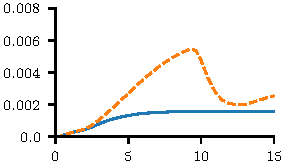
\includegraphics[width=1.0\linewidth]{param_study/v-4r-3_kinetic_energy.pdf}
      \caption{$\nu = 10^{-4};\ \eta = 10^{-3}$}%
      \label{fig:v-4r-3_kinetic_energy_ps}
    \end{subfigure}
    \hfill
    \begin{subfigure}{0.32\textwidth}
      \centering
      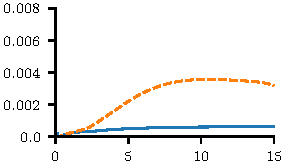
\includegraphics[width=1.0\linewidth]{param_study/v-3r-3_kinetic_energy.pdf}
      \caption{$\nu = 10^{-3};\ \eta = 10^{-3}$}%
      \label{fig:v-3r-3_kinetic_energy_ps}
    \end{subfigure}
    \hfill
    \begin{subfigure}{0.32\textwidth}
      \centering
      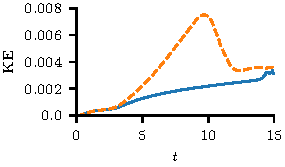
\includegraphics[width=1.0\linewidth]{param_study/v-5r-4_kinetic_energy.pdf}
      \caption{$\nu = 10^{-5};\ \eta = 10^{-4}$}%
      \label{fig:v-5r-4_kinetic_energy_ps}
    \end{subfigure}
    \hfill
    \begin{subfigure}{0.32\textwidth}
      \centering
      \includegraphics[width=1.0\linewidth]{param_study/v-4r-4_kinetic_energy.pdf}
      \caption{$\nu = 10^{-4};\ \eta = 10^{-4}$}%
      \label{fig:v-4r-4_kinetic_energy_ps}
    \end{subfigure}
    \hfill
    \begin{subfigure}{0.32\textwidth}
      \centering
      \includegraphics[width=1.0\linewidth]{param_study/v-3r-4_kinetic_energy.pdf}
      \caption{$\nu = 10^{-3};\ \eta = 10^{-4}$}%
      \label{fig:v-3r-4_kinetic_energy_ps}
    \end{subfigure}
  %
\includegraphics[width=\linewidth]{param_study/kinetic_energies.pdf}
  \caption{Kinetic energy against time for each parameter choice and each viscosity model. An increase in $\nu$ damps the energy released during the KHI in the switching cases and totally suppresses the KHI in most isotropic cases.}%
  \label{fig:param_study_kinetic_energies}
\end{figure}

Figure~\ref{fig:param_study_kinetic_energies} shows the kinetic energy as a function of time for all parameter choices and both viscosity models. The strongly KHI-unstable cases show a similar kinetic energy profile to that of the typical cases (Figure~\ref{fig:v-4r-4_kinetic_energy}). In the switching cases, the peak kinetic energy is larger when $\eta=10^{-4}$ in two cases (Figures~\ref{fig:v-5r-4_kinetic_energy_ps} and~\ref{fig:v-4r-4_kinetic_energy_ps}). This is a result of the reduced diffusion of the magnetic field resulting in a stronger vorticity layer (Figure~\ref{fig:param_study_peak_mag_and_loc}). The isotropic cases in Figure~\ref{fig:param_study_kinetic_energies} show an interesting trend in that the kinetic grows more for smaller $\nu$ (as expected) or for larger $\eta$. In particular, the isotropic case where $\eta=10^{-3}$ and $\nu=10^{-5}$ (Figure~\ref{fig:v-5r-3_kinetic_energy_ps}) is only isotropic case where the KHI is significantly unstable. In this case the kinetic energy profile shares a similar shape to the associated switching case, but the enhanced dissipation prevents the KHI from generating similar levels of kinetic energy. Instead, the profile is much flatter and saturates at a later time.

Table~\ref{tab:stability} reveals three cases of interest which can be explored through the kinetic energy profiles. The marginally unstable isotropic case, where $\eta=10^{-4}$ and $\nu=10^{-5}$, does show some growth but it is notably less than the fully unstable case (Figure~\ref{fig:v-5r-4_kinetic_energy_ps}). Given that the current-vortex sheets in both these cases share similar strengths of vorticity, it is the combination of viscous dissipation of perturbations and enhanced magnetic shear in the lower $\eta$ case which acts to stabilise the sheet (Figure~\ref{fig:param_study_peak_mag_and_loc}). This conclusion can similarly be drawn for the outlying switching case where $\eta=10^{-4}$ and $\nu=10^{-3}$ (Figure~\ref{fig:v-3r-4_kinetic_energy_ps}). The remaining case of interest is where $\eta=10^{-3}$ and $\nu=10^{-4}$, the single case where the linear prediction disagrees with the observed stability (Figure~\ref{fig:v-4r-3_kinetic_energy_ps}). In this case, the kinetic energy plateaus as the viscosity dissipates kinetic energy as it is generated by the instability.

\begin{figure}[t]
    \hfill
    \begin{subfigure}{0.32\textwidth}
      \centering
  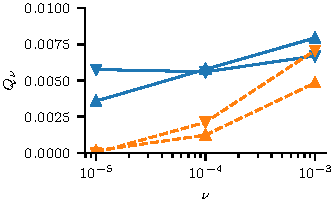
\includegraphics[width=1.0\linewidth]{param_study/final_visc_heating.pdf}
      \caption{Viscous heating}%
      \label{fig:ps_visc_heating}
    \end{subfigure}
    \hfill
    \begin{subfigure}{0.32\textwidth}
      \centering
  \includegraphics[width=1.0\linewidth]{param_study/final_ohmic_heating.pdf}
      \caption{Ohmic heating}%
      \label{fig:ps_ohmic_heating}
    \end{subfigure}
    \hfill
    \begin{subfigure}{0.32\textwidth}
      \centering
  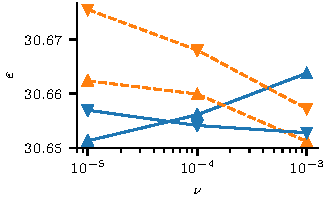
\includegraphics[width=1.0\linewidth]{param_study/final_internal_energy.pdf}
      \caption{Internal energy}%
      \label{fig:ps_interal_energy}
    \end{subfigure}
  \caption{Plots of internal energy, total viscous and total Ohmic heat as functions of $\nu$ at $t=12.5$, before the onset of any null collapse, for all parameter choices. Isotropic (blue, solid) and switching viscosity (orange, dashed) are both shown. An upwards-facing triangle denotes the higher value of $\eta=10^{-3}$ and a downwards-facing triangle, $\eta=10^{-4}$. The anisotropic viscous heating can become significant for larger values of $\nu$ yet, when $\nu$ is smaller, the lack of viscous heating is compensated by enhanced Ohmic heating. }%
  \label{fig:ps_heating}
\end{figure}

Figure~\ref{fig:ps_heating} presents the total heat generated by viscous and Ohmic dissipation and the total internal energy at $t=13$, prior to any null collapse. Looking first at the viscous heating (Figure~\ref{fig:ps_visc_heating}), $Q_{\nu}$ generally decreases with decreasing $\nu$, as one may expect, with the exception of the isotropic cases where $\eta=10^{-4}$. Instead, in these cases the viscous heating shows little dependence on $\nu$. This reveals the complex, nonlinear relationship between viscous heating, the value of $\nu$ and the flows generated.

In the switching cases, generally an increase in $\nu$ increases viscous heating and decreases Ohmic heating. The decrease in Ohmic heating is due to two complementary effects. Firstly, viscosity generally slows flows and limits the compression of current sheets, consequently limiting Ohmic heating, thus a larger $\nu$ produces less Ohmic heating. Secondly, the nonlinear phase of the KHI enhances Ohmic heating in the fan plane and, since the instability is more unstable for smaller $\nu$, Ohmic heating increases with decreasing $\nu$. The overall effect is a decrease in internal energy with increasing $\nu$. This is also true for the $\eta=10^{-3}$ isotropic cases.

The Ohmic heating profile similarly reveals complex behaviour in the isotropic cases (Figure~\ref{fig:ps_ohmic_heating}. The stark difference in trends can be explained by considering the spatial distribution of Ohmic heating which mirrors that of the current density. The two main current structures in a twisted null are the current-vortex sheet and the structure associated with the twisted spines (although the spine currents are two separate regions of current density, they contribute equally to the Ohmic heating so are considered one here). These are the main sources of Ohmic heating and the balance of contributions from each source, for different values of $\eta$ and $\nu$, is non-trivial and results in the observed difference in trends.

\begin{figure}[t]
  \begin{subfigure}{0.49\textwidth}
      \centering
  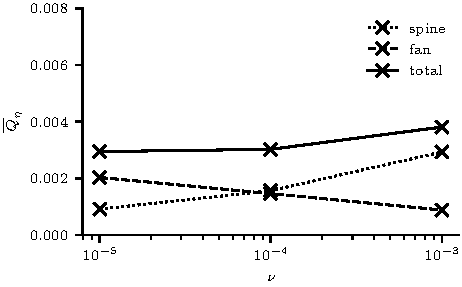
\includegraphics[width=1.0\linewidth]{param_study/balance_of_ohmic_heating-3.pdf}
      \caption{$\eta = 10^{-3}$}%
      \label{fig:balance_of_ohmic_heating-3}
    \end{subfigure}
    \hfill
    \begin{subfigure}{0.49\textwidth}
      \centering
  \includegraphics[width=1.0\linewidth]{param_study/balance_of_ohmic_heating-4.pdf}
      \caption{$\eta = 10^{-4}$}%
      \label{fig:balance_of_ohmic_heating-4}
    \end{subfigure}
  \caption{Mean Ohmic heating contributions from the spines (dotted) and current-vortex sheet (dashed) and their sum (solid) for $\eta=10^{-3}$ (a) and $\eta=10^{-4}$ (b) in only the isotropic cases at $t=10$. The value of $\eta$ dictates how rapidly the balance of contributions shifts from fan to spine with $\nu$, resulting in different trends in total Ohmic heating.}%
  \label{fig:balance_of_ohmic_heating}
\end{figure}

Figure~\ref{fig:balance_of_ohmic_heating} reveals how the contributions from the current-vortex sheet and spines change with $\nu$, and the effect that has on the total Ohmic heating. These measures are calculated as the mean of the Ohmic heating in the $xy$-plane (representing the heating within the current-vortex sheet) and that in the $yz$-plane (representing the heating in the spines). These are not true measurements of the Ohmic heating within each current structure, however they provide a useful proxy. 

For any value of $\eta$, the spine heating increases and the current-vortex heating decreases as $\nu$ increases. This is due to greater viscosity dissipating the initial Alfv\'en waves more effectively and reducing the magnetic shear in the current-vortex sheet while retaining magnetic shear in the spines. The difference in how rapidly the relative contributions change with $\nu$ gives rise to the difference in total Ohmic heating trends found in Figure~\ref{fig:ps_ohmic_heating}. When $\eta=10^{-4}$, the heating in the sheet decreases faster than the spine heating increases with $\nu$, resulting in a drop in total Ohmic heating (Figure~\ref{fig:balance_of_ohmic_heating-4}). The opposite is true when $\eta=10^{-3}$ (Figure~\ref{fig:balance_of_ohmic_heating-3}).

\section{Discussion}
\label{sec:khi_discussion}

While the values of $\eta$ used in the simulations performed here are orders of magnitude greater than typical coronal estimates, the values of $\nu$ are certainly within realistic bounds. It has been found that, when using a model of viscosity appropriate in the solar corona, i.e. the switching model, the KHI is unstable, regardless of parameter choice. This strongly suggests that, in the real corona, the KHI can be excited in current-vortex sheets such as those studied here. What this investigation does not take into account are other possible null point configurations.

This chapter details the investigation of the KHI and null point collapse around an axisymmetric, linear null point, an idealised model of a real null point (such as that observed in~\cite{massonNATUREFLARERIBBONS2009}). The impact of non-ideal null configurations such as those with asymmetry (e.g. those investigated in~\cite{thurgoodImplosiveCollapseMagnetic2018,pontinWhyAreFlare2016a}) is unclear. Similarly, the simplicity of the driver used here is unlikely to reflect the true nature of drivers in the real solar corona. The impact of driver complexity on spine-fan reconnection specifically has been investigated~\cite{wyperSpinefanReconnectionInfluence2012}, however the drivers studied in~\cite{wyperSpinefanReconnectionInfluence2012} only sheared the field (as opposed to the torsional drivers employed here). It would be of interest to understand how different magnetic field configurations and forms of driver affect the formation and stability of the kinds of current-vortex sheets studied here.

The simulations detailed here have been performed with a model of anisotropic viscosity which only captures the parallel component of viscosity. As discussed in~\cite{einaudiResistiveInstabilitiesFlowing1989}, perpendicular components can become significant in strong velocity shears (such as those found in the fan plane of a twisted null point) despite the small size of the associated transport coefficient $\eta_1$ (see section~\ref{sec:braginskii_tensor}). A similar set of experiments exploring the effect of the perpendicular viscosity could provide useful insight, particularly in ascertaining if the growth of the tearing instability in the current-vortex sheet could be accelerated by perpendicular viscosity, as is found in the linear analysis performed by~\cite{einaudiResistiveInstabilitiesFlowing1989}.

An important, unexpected finding of this investigation is the spontaneous collapse of the null point without shearing drivers (as in~\cite{pontinCurrentSheetFormation2007}) or prescribed current density perturbations (as in~\cite{thurgoodImplosiveCollapseMagnetic2018}). The primary drivers of the shearing motion above and below the null (which gives rise to a current sheet, associated spine-fan reconnection and eventual collapse) are the oppositely directed streams of plasma flowing along the spines towards the null. These flows rely on the pressure gradients which are generated by Ohmic heating in the twisted spines. In chapter~\ref{chp:kink_instability_straight} it was found that the pressure generated in the ideal case (i.e. without any Ohmic heating) was too small to generate a fluting instability. Similarly, here, it may be that the pressure generated under ideal conditions (or using realistically small coronal resistivity) is not enough to drive the null-directed flows and, thus, not enough to collapse the null. Further investigation of this form of collapse within a twisted null point is required to ascertain if such a collapse is possible in the real corona.

The effect of the form of viscosity on the collapse of the null is also explored in the two high-resolution simulations (of Section~\ref{sec:null_point_khi_single_case}) and it is found that in the switching case, where the KHI is unstable, the null collapses notably earlier than in the isotropic case, where the KHI is stable. It is unclear if the early null collapse is a consequence of the KHI or the use of the switching model. From the results of the isotropic case, the null collapse appears to be ultimately caused by slight asymmetries in the spine-aligned flows, so one may conjecture that, in the switching case, the KHI introduces its own asymmetries which cause the early collapse of the null. A higher resolution version of the unstable, isotropic case (where $\nu = 10^{-5}$ and $\eta=10^{-3}$) would provide clarity and provides an avenue of further study.

It is unclear how the unravelling of the null as it collapses affects the ability of the null to undergo the kind of oscillatory reconnection found in~\cite{thurgoodThreedimensionalOscillatoryMagnetic2017}. One observed phase in the oscillatory process is the generation of back-pressure which halts and reverses the spine-fan reconnection process. It may be that a collapsing twisted null is unable to produce the required back-pressure if it unravels during its initial collapse. Running the high-resolution simulations reported here for a longer time would reveal if the particular setup studied here can generate oscillatory spine-fan reconnection. Alternatively, using a pre-twisted null point as an initial condition with the perturbation used to collapse the null found in~\cite{thurgoodThreedimensionalOscillatoryMagnetic2017} would provide a similar experiment.

%\subsubsection{Limitations of the simulations}

%In many of the results presented, the effect of the boundaries is small but apparent (for instance, where the KHI first appears along the diagonals of the $x-y$ plane) despite the use of a damping layer. 

%In the simulations performed here, the resolution was set such that the same number of grid points were used in each direction. In hindsight, the resolution could have been better balanced by using more grid points in the relatively long $x$ and $y$ directions than the relatively short $z$ direction, although this would have impacted the resolution across the shear layers. A non-uniform grid could have been used, with higher resolution focused near the null point. This is commonly done in other studies of null point dynamics~\cite{wyperKelvinHelmholtzInstabilityCurrentvortex2013,thurgoodThreedimensionalOscillatoryMagnetic2017}.

\section{Conclusions}
\label{sec:khi_conclusions}

In this chapter I have compared two models of viscosity applied to a magnetic null point which has been dynamically twisted at its footpoints in such a way that a current-vortex sheet forms in the fan plane. This sheet has the potential to become unstable to the KHI. It was found that increased viscous dissipation, particularly in the form of isotropic viscosity, has a stabilising effect on the sheet. This is primarily due to viscosity thickening the sheet and increasing its stability. The presence of the instability enhances reconnection locally within the sheet.

After some time, the null spontaneously collapses due to an imbalance in spine-directed, pressure-driven flows. This is found to occur sooner when the KHI is present. The general development of the collapse and associated spine-fan reconnection is similar to that of previous work with the exception that the twist in the spines unravels during the collapse.

The investigation of the stability of the current-vortex sheet was extended with a parameter study over an order of magnitude difference in resistivity and two in viscosity. The results show that the KHI is mostly unstable when using switching viscosity and mostly stable when using isotropic viscosity.
